\section{Параллельные алгоритмы -- i (Осипов Д.)}

Параллельный алгоритм -- предназначенный для исполнения на нескольких процессах. 
\subsection{Булевы схемы как модель параллельного алгоритма}
\statement{Определение.}{Булева схема} -- ориентированный граф без циклов, где: 
\begin{itemize}
    \item вершины без входящих ребер соответствуют входным данным,
    \item вершины с входящими ребрами (<<гейты>>) соответствуют процессорам, которые выполняют операцию с данными, поступающими в вершину по входящим ребрам,
    \item вершины без выходящих ребер соответствуют выходным данным.
\end{itemize}
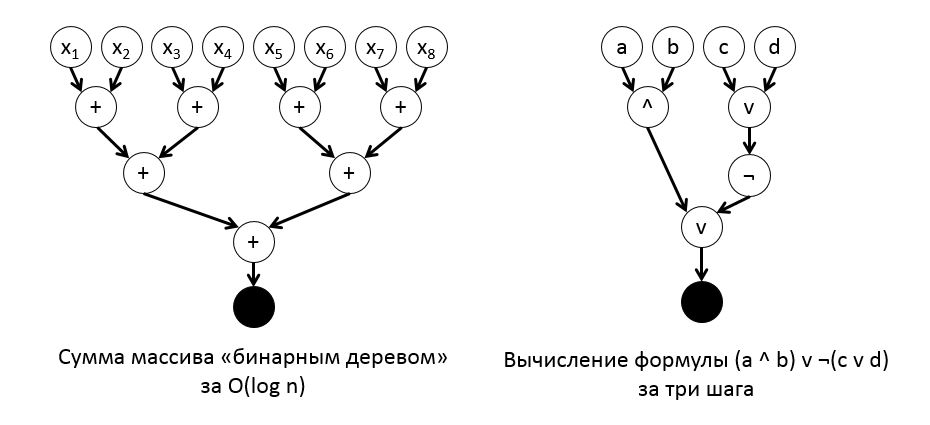
\includegraphics[scale=0.5]{figures/boolex.jpg}
 
\textit{<<Высота>>} схемы, т.е. длина наибольшего пути от вершины выходных данных -- количество параллельных шагов алгоритма. Еще можно заметить, что если каждому гейту присвоить число -- <<номер этажа>> так, что каждый переход осуществляется с <<верхнего>> этажа на <<нижний>>, то максимальное число процессоров на одном этаже -- достаточное количество процессоров для исполнения всего алгоритма. Так, в левом примере достаточно взять четыре процессора, а в правом -- два. 

Суммирование массива за $O(\log n)$ параллельных шагов в примере слева -- уже хороший пример параллельного алгоритма. Хотя он интуитивно понятен, опишем его формально. 

\statement{Задача.}{Пусть дано $n$ чисел. Вычислить их сумму.}

\statement{Решение за $O(\log n).$}{} Считаем, что $n$ -- степень двойки (если нет, дополним нулями).  Разобъем все числа на $n/2$ пар и поручим каждому процессору одну пару, чтобы он вычислил ее сумму. Получившиеся $n/2$ чисел разобъем на $n/4$ пар и так же вычислим суммы этих пар. Повторяем до тех пор, пока не останется одно число. Ясно, что всего будет выполнено $\log_2 n = O(\log n)$ параллельных шагов. \qed

\statement{NB:}{ Сложить\footnote{Имея в распоряжении только <<+>>-гейты, принимающие ровно два числа} $n$ чисел быстрее, чем за $\log n$ шагов, нельзя.} В самом деле, если можно, то булева схема такого алгоритма как граф-дерево имеет высоту $h \leq \log_2 n - 1$. Но каждый гейт принимает на вход не больше двух чисел, т.е. входная степень каждой вершины не больше 2. Значит верхних входных гейтов не может быть более $2^h \leq n/2$  чисел, а надо $n$.

При проектировании параллельных алгоритмов в качестве меры их эффективности возникает аж три параметра: \textit{количество параллельных шагов (время работы)}, \textit{количество используемых процессоров} и \textit{общая работа} (определение дано далее). К счастью, об одном из них -- количестве процессоров -- можно не задумываться, о чем говорит нам следующее утверждение.

\subsection{Принцип Брента}
\statement{Теорема (принцип Брента).}{Рассмотрим параллельный алгоритм, выполняющий t параллельных шагов, где на $i-$том шаге задействовано $w_i$ процессоров (т.е. выполняется $w_i$ операций). Обозначим $W=\sum\limits_{i=1}^t w_i$ и назовем эту величину \underline{общей работой алгоритма}. Тогда алгоритм можно перепрограммировать так, чтобы на $P$ процессорах он работал не более, чем за $\frac{W}{P} + t$ параллельных шагов.}

\statement{Доказательство.}{} Перераспределим все $W$ операций на $P$ процессорах наиболее равномерно. Тогда $i$-тый шаг изначального алгоритма можно выполнить за $\left\lceil\frac{w_i}{P}\right\rceil$ новых шагов. Оценим общее число шагов нового алгоритма:
$$t' = \sum_{i=1}^t \left\lceil\frac{w_i}{P}\right\rceil \leq \sum_{i=1}^t \left(\frac{w_i}{P} + 1\right) = \sum_{i=1}^t \frac{w_i}{P} + t = \frac{W}{P} + t$$Таким образом, получили алгоритм с искомым временем работы. \qed

\statement{NB: }{} Принцип Брента позволяет при проектировании параллельных алгоритмов \textbf{не думать}, на скольких процессорах будет работать алгоритм. Именно: пусть был создан алгоритм, работающий на неизвестном (лень считать) числе процессоров $P_0(n)$ и совершающий общую работу $W(n)$ за $t(n)$ параллельных шагов. Тогда его можно перепроектировать на любое число процессоров $P(n)$ такое, что $$\frac{W(n)}{P(n)} = O(t(n)),$$ и асимптотически не потерять во времени, так как тогда новое время работы все еще $t'(n) \leq \frac{W(n)}{P(n)} + t(n) = O(t(n))$. Поэтому в дальнейшем при изучении параллельных алгоритмов считаем, что у нас \textbf{сколь угодно много процессоров}, а затем количество нужных процессоров будем вычислять по принципу Брента.

\subsection{Параллельное умножение булевых матриц}
\statement{NB:}{ булевые -- только чтобы арифметика с числами была $O(1)$.}

\statement{Задача.}{Даны две матрицы $A$ и $B$ размера $n\times n$ над $\mathbb F_2$. Вычислить их произведение, то есть числа $C_{ij} = \sum_{k=1}^n A_{ik}B_{kj}$  для всех $i, j=1..n$ (всего $n^2$  чисел)}.

\statement{Непараллельное решение.}{} Вычислить все $n^2$ чисел $C_{ij}$, каждое считается за $O(n)$, значит общая сложность $O(n^3)$.  \qed

Несмотря на то, что в прошлом разделе мы условились не думать о количестве процессоров, конкретно здесь на всякий случай приведем два решения. Второе решение -- просто пример того, как работает принцип Брента. 

\statement{Решение за $O(\log n)$ времени на $n^3$ процессорах.}{} Занумеруем все $n^3$ процессоров тройками чисел $(i, k, j)$, где $i,k,j=1..n$. Сначала на каждом процессоре $(i, k, j)$ посчитаем $A_{ik}B_{kj}$. Теперь хотим получить число $C_{ij} = \sum_{k=1}^n (i, k, j)$, Сделаем это за $\log n$ шагов (суммирование бинарным деревом). Задача решена за $1+\log n = O(\log n) $ шагов на $n^3$ процессорах. \qed

\textit{\underline{Вместо второго решения}, можно, наверное, просто привести первое решение, а затем вычислить оптимально возможное количество процессоров, на которое это решение можно перепроектировать.} Общая работа этого решения $W(n) = O(n^3)$. Действительно, ведь данное решение просто считает $n^2$ сумм $C_{ij} = \sum_{k=1}^n A_{ik}B_{kj}$, переставив слагаемые в другом порядке, таким образом, $n^2$ раз совершено $n$ действий сложения. Тогда количество процессоров $P$ вычисляется из $\frac{W(n)}{P(n)} = O(t(n)) \implies P(n) = \frac{W(n)}{t(n)} = O\left(\frac{n^3}{\log n}\right)$

\statement{Решение за $O(\log n)$ времени на $O\left(\frac{n^3}{\log n}\right)$ процессорах.}{} Модифицируем алгоритм выше. На первом шаге вычислить все числа $A_{ik}B_{kj}$ получится не за 1, а за $O(\log n)$ шагов: за каждый шаг просто посчитаются очередные $\frac{n^3}{\log n}$ чисел $A_{ik}B_{kj}$. Получать из них $C_{ij}$ за $O(\log n)$ мы уже умеем. Итоговая сложность $O(\log n) + O(\log n) = O(\log n)$.  \qed

\subsection{Параллельная достижимость в графе}
\statement{Задача.}{Дан граф, заданный матрицей смежности $\{a_{ij}\}$. Построить его матрицу достижимости.} 

\statement{Решение за $O(\log^2 n)$ времени}{} Будем булево умножать матрицы: вместо $\cdot$ возьмем $\land$, вместо $+$ возьмем $\lor$. Из формулы перемножения матриц несложно видеть, что $A^k$ -- матрица $k-$шаговой достижимости. Тогда матрица достижимости -- любая матрица $A^k$, где $k\geq n$. Умеем возводить матрицу в квадрат за $O(\log n)$. Для получения матрицы достижимости $A^n$. возведем матрицу $A$ в квадрат $\log n$ раз. Итоговая сложность $O(\log n) \cdot O(\log n) = O(\log^2 n)$. Общая работа W(n) = $O(n^3\log n)$, так как $\log n$ раз перемножили матрицы за $O(n^3)$ работы. Число процессоров: $P(n) = O(\frac{n^3\log n}{\log^2 n}) = O(\frac{n^3}{\log n})$. \qed
